\section{Наиболее употребимые теоретические законы распределения вероятностей. Примеры и свойства распределений для дискретных и непрерывных величин}

В теории вероятностей \textbf{закон распределения} случайной величины описывает, какие значения она может принимать и с какой вероятностью.  
Все законы делятся на два больших класса: \textbf{дискретные} и \textbf{непрерывные}.

\subsection{Дискретные законы распределения}

Дискретная случайная величина может принимать конечное или счётное число значений. Закон распределения задаётся таблицей или функцией вероятности:
\[
P(X = x_i) = p_i, \quad p_i \geq 0, \quad \sum_{i} p_i = 1.
\]

\subsubsection{Распределение Бернулли}
Описывает исход одного эксперимента с двумя результатами: ``успех'' (1) с вероятностью $p$ и ``неудача'' (0) с вероятностью $q = 1 - p$.
\[
P(X = 1) = p, \quad P(X = 0) = 1 - p.
\]
\textbf{Математическое ожидание:} $E[X] = p$.  
\textbf{Дисперсия:} $D[X] = p(1-p)$.

\begin{center}
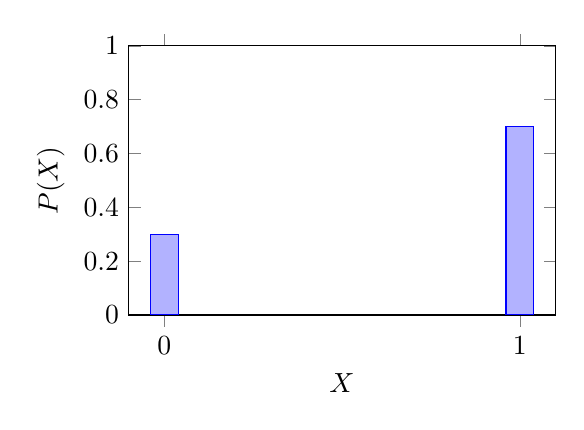
\begin{tikzpicture}
\begin{axis}[
    ybar,
    symbolic x coords={0,1},
    xtick=data,
    ymin=0, ymax=1,
    xlabel={$X$}, ylabel={$P(X)$},
    width=7cm, height=5cm
]
\addplot coordinates {(0,0.3) (1,0.7)};
\end{axis}
\end{tikzpicture}
\end{center}

\subsubsection{Биномиальное распределение}
Описывает количество успехов в $n$ независимых испытаниях Бернулли с вероятностью успеха $p$.
\[
P(X = k) = \binom{n}{k} p^k (1-p)^{n-k}, \quad k = 0,1,\dots,n.
\]
\textbf{Математическое ожидание:} $E[X] = np$.  
\textbf{Дисперсия:} $D[X] = np(1-p)$.

\begin{center}
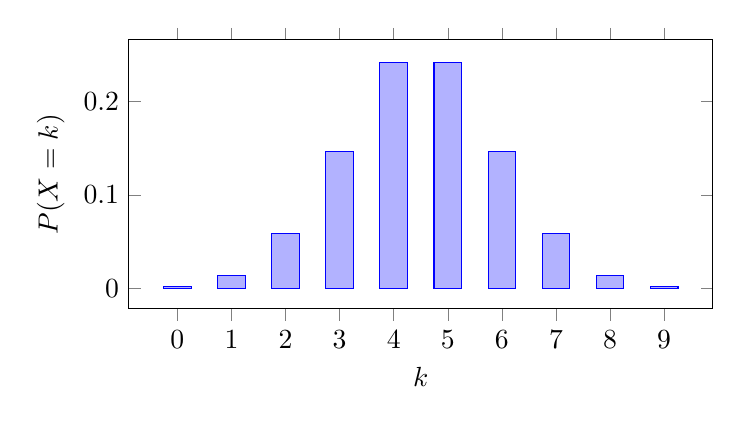
\begin{tikzpicture}
\begin{axis}[
    ybar,
    xtick=data,
    xlabel={$k$}, ylabel={$P(X=k)$},
    width=9cm, height=5cm
]
\addplot coordinates {
(0,0.002) (1,0.014) (2,0.059) (3,0.146) (4,0.242) (5,0.242) (6,0.146) (7,0.059) (8,0.014) (9,0.002)
};
\end{axis}
\end{tikzpicture}
\end{center}

\subsubsection{Геометрическое распределение}
Вероятность того, что первый успех произойдёт на $k$-м испытании:
\[
P(X = k) = (1-p)^{k-1}p, \quad k = 1,2,3,\dots
\]
\textbf{Математическое ожидание:} $E[X] = \frac{1}{p}$.  
\textbf{Дисперсия:} $D[X] = \frac{1-p}{p^2}$.

\subsection{Непрерывные законы распределения}

Непрерывная случайная величина может принимать любое значение на отрезке или на всей числовой прямой.  
Её распределение задаётся функцией плотности вероятности $f(x)$, удовлетворяющей условиям:
\[
f(x) \geq 0, \quad \int_{-\infty}^{\infty} f(x)\,dx = 1.
\]

\subsubsection{Равномерное распределение}
Если случайная величина $X$ равновероятно принимает значения на отрезке $[a,b]$, то
\[
f(x) = \frac{1}{b-a}, \quad a \leq x \leq b.
\]
\textbf{Математическое ожидание:} $E[X] = \frac{a+b}{2}$.  
\textbf{Дисперсия:} $D[X] = \frac{(b-a)^2}{12}$.

\begin{center}
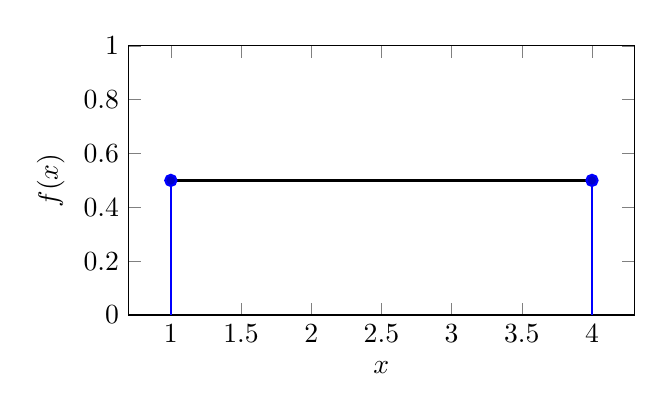
\begin{tikzpicture}
\begin{axis}[
    xlabel={$x$}, ylabel={$f(x)$},
    width=8cm, height=5cm,
    ymin=0, ymax=1
]
\addplot+[ycomb, thick] coordinates {(1,0.5) (4,0.5)};
\addplot[domain=1:4, samples=2, thick] {0.5};
\end{axis}
\end{tikzpicture}
\end{center}

\subsubsection{Нормальное распределение}
Наиболее распространённое в природе и статистике.  
Функция плотности:
\[
f(x) = \frac{1}{\sigma \sqrt{2\pi}} e^{-\frac{(x-\mu)^2}{2\sigma^2}}, \quad -\infty < x < \infty.
\]
\textbf{Математическое ожидание:} $E[X] = \mu$.  
\textbf{Дисперсия:} $D[X] = \sigma^2$.

\begin{center}
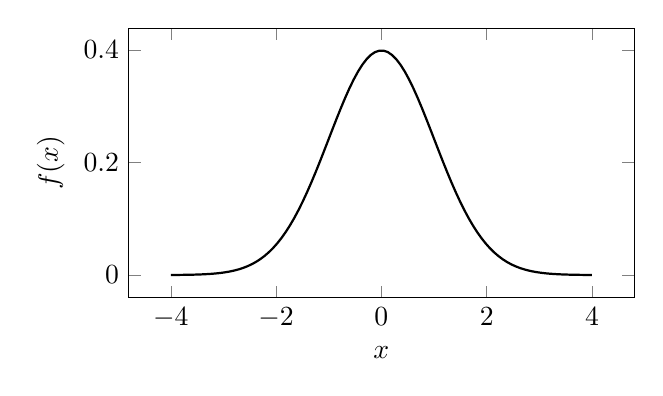
\begin{tikzpicture}
\begin{axis}[
    xlabel={$x$}, ylabel={$f(x)$},
    width=8cm, height=5cm
]
\addplot[domain=-4:4, samples=100, thick] {1/sqrt(2*pi) * exp(-x^2/2)};
\end{axis}
\end{tikzpicture}
\end{center}

\subsubsection{Экспоненциальное распределение}
Часто описывает время ожидания между событиями.
\[
f(x) = \lambda e^{-\lambda x}, \quad x \geq 0.
\]
\textbf{Математическое ожидание:} $E[X] = \frac{1}{\lambda}$.  
\textbf{Дисперсия:} $D[X] = \frac{1}{\lambda^2}$.

\begin{center}
\begin{tikzpicture}
\begin{axis}[
    xlabel={$x$}, ylabel={$f(x)$},
    width=8cm, height=5cm
]
\addplot[domain=0:5, samples=100, thick] {exp(-x)};
\end{axis}
\end{tikzpicture}
\end{center}

\subsection{Выводы и сравнение}
Каждое распределение имеет свои особенности и применяется в определённых задачах:
\begin{itemize}
    \item Бернулли и биномиальное --- для дискретных экспериментов с успехами и неудачами.
    \item Геометрическое --- для моделирования числа попыток до первого успеха.
    \item Равномерное --- когда все значения равновероятны.
    \item Нормальное --- в большинстве природных и социальных явлений.
    \item Экспоненциальное --- для моделирования времени ожидания.
\end{itemize}
